%! suppress = MissingLabel

Продолжения с начала 60х не один раз возникали в литературе в различных формах и разнообразных приложениях~\cite{reynolds1993discoveries, landin1997histories}, пока в 70х Wadsworth не придумал общий термин и единую концепцию --- \vocab{continuation}\footnote{\url{https://en.wikipedia.org/wiki/Continuation}} --- ``the meaning of the rest of the program''.

Начальным толчком к размышлениям стал язык Algol 60, имевший нетривиальный механизм меток и прыжков.
Проблемой была как имплементация семантики, так и её денотационное описание вместе с трансляцией в лямбда-исчисление.
Действительно, как математически описать \texttt{goto}?
В каком домене искать семантику таких программ?
Как написать определяющий интерпретатор, отправляющий программу в этот домен?
Ответом стала возможность сослаться на семантику остатка программы в определённой точке (например, на метке).

Итак, продолжение --- это абстрактная концепция, обозначающая остаток вычисления.
Например, когда мы редуцируем простое арифметическое выражение, вычислитель фокусируется внутрь его, чтобы найти редекс.
Оставшееся выражение с дыркой, в которую нужно будет подставить результат вычисления редекса, является продолжением.

\begin{figure}[h]
    \centering
    \begin{tabular}{|c|c|}
        \hline
        Фокус               & Продолжение           \\
        \hline
        $((2 + 3) - 4) * 5$ & $\boxempty$           \\
        $(2 + 3) - 4$       & $\boxempty * 5$       \\
        $2 + 3$             & $(\boxempty - 4) * 5$ \\
        $5$                 & $(\boxempty - 4) * 5$ \\
        $5 - 4$             & $\boxempty * 5$       \\
        $1$                 & $\boxempty * 5$       \\
        $1 * 5$             & $\boxempty$           \\
        $5$                 & $\boxempty$           \\
        \hline
    \end{tabular}
\end{figure}

Практически говоря, продолжение представляет собой некоторую структуру данных, сохраняющее всё что нужно, чтобы продолжить исполнение программы с определённого места.
Иначе говоря, это некоторый снапшот состояния вычислителя, интерпретатора.

Как правило, продолжения существуют вне пользовательского кода.
Это разработчику системы исполнения языка нужно думать, хранение чего нужно поддержать, чтобы продолжать исполнять программу в каждый момент.
Однако, современные языки предоставляют пользователям множество конструкций, позволяющих управлять продолжениями:

\begin{itemize}
    \item Функция \mintinline{haskell}|exit| выбрасывает продолжение программы целиком;
    \item Конструкция \mintinline{kotlin}|try-catch| позволяет выбросить часть продолжения до места поимки исключения и восстановить доставшееся;
    \item Конструкция \mintinline{kotlin}|return| позволяет восстановить исполнение в месте, где функция была вызвана;
    \item Конструкции \mintinline{kotlin}|break| и \mintinline{kotlin}|continue| восстанавливают продолжение после цикла и до\ldots
\end{itemize}

В примерах выше конструкции языка управляют продолжениями неявно.
Однако, иногда вводят операторы, позволяющие явно оперировать продолжениями.

\vocab{Продолжения первого класса (first-class continuations)} --- продолжения, которые представимы в программе в виде значений.
Учитывая, что продолжение имеет вакантное место ещё не вычисленного подвыражения, продолжения первого класса представляют функциями первого класса.

Чтобы получить в коде продолжение первого класса, нужно либо написать код в специальном виде, либо воспользоваться встроенным в язык оператором~\cite[приложение A]{hillerstrom2022foundations}.
Например, $J$, \texttt{escape}~\cite{reynolds1972definitional}, \texttt{call/cc}\ldots

\subsection{Continuation-passing style (CPS)}

Базовым способом получить в программе продолжение первого класса --- написать программу в стиле CPS.
CPS эксплуатирует следующий изоморфизм:
\begin{minted}{haskell}
    to :: a -> (forall r . (a -> r) -> r)
    to x k = k x

    from :: (forall r . (a -> r) -> r) -> a
    from comp = comp id
\end{minted}

Иначе говоря, вместо того, чтобы предоставить значение, можно запросить у вызывающей стороны, как она собирается с этим значением работать, сделать это самостоятельно и вернуть вызывающей стороне\footnote{\url{https://wiki.haskell.org/Cont_computations_as_question-answering_boxes}}.

Корни этого изоморфизма в лемме Йонеды из теории категорий~\cite{hinze2010reason}.
Прикладным же программистам он знаком по технике использования callback'ов.

Например, мы можем переписать факториал в стиле CPS.
Заметьте, что код имеет доступ к продолжению первого класса (однако, никак нетривиально не использует его).
\begin{minted}{haskell}
    facCps :: Int -> (forall r . (Int -> r) -> r)
    facCps n k
      | n <= 1 = k 1
      | otherwise = facCps (n - 1) \res -> k (n * res)
\end{minted}

\begin{task}
    Вручную поредуцируйте определение \mintinline{haskell}|facCps| на простом примере.
\end{task}

\begin{task}
    Сколько функция \mintinline{haskell}|facCps| потребляет стековой памяти?
\end{task}

\subsubsection{Монада \texttt{Cont}}

Из-за CPS код потерял привычную структуру, при которой функции напрямую возвращают свои результаты.
При наличии большого количества вызовов трансформированных функций, код становится плохо читаемым.

\begin{minted}{haskell}
    fibCps :: Int -> (forall r . (Int -> r) -> r)
    fibCps n k = if n <= 2 then k 1 else
      fibCps (n - 1) \res1 ->
      fibCps (n - 2) \res2 ->
      k (res1 + res2)
\end{minted}

Однако, можно заметить, что монадическое связывание вторым аргументом тоже принимает продолжение, но ``маленькое'', до конца \mintinline{haskell}|do|-блока.
Таким образом, можно попробовать линеаризовать CPS код с помощью монад.

Заведём \mintinline{haskell}|newtype| обёртку для объявления инстансов:
\begin{minted}{haskell}
    newtype Cont r a = Cont { runCont :: (a -> r) -> r }
\end{minted}

Функтор добавляет пост-процессинг результату перед передачей в продолжение:
\begin{minted}{haskell}
    instance Functor (Cont r) where
      -- fmap :: (a -> b) -> ((a -> r) -> r) -> ((b -> r) -> r)
      fmap f (Cont comp) = Cont \k -> comp (k . f)
\end{minted}

Аппликатив просто передаёт значение продолжению:
\begin{minted}{haskell}
    instance Applicative (Cont r) where
      pure x = Cont \k -> k x
      (<*>) = ap
\end{minted}

Наконец, монада принимает в связывании ``маленькое'' продолжение, композирует его с ``большим'' продолжением, пришедшим снаружи, и передаёт в данное вычисление:
\begin{minted}{haskell}
    instance Monad (Cont r) where
      Cont comp >>= k = Cont \k' -> comp \x -> runCont (k x) k'
\end{minted}

Теперь мы можем писать линейный код, а монадическая машинерия сама конструирует продолжения и подкладывает в предыдущие вычисления:
\begin{minted}{haskell}
    fibCont :: Int -> Cont r Int
    fibCont n = if n <= 2 then pure 1 else do
      res1 <- fibCont (n - 1)
      res2 <- fibCont (n - 2)
      pure (res1 + res2)
\end{minted}

\begin{task}
    Оборвите вычисление, если \texttt{res1} больше \texttt{50}.
\end{task}

\begin{task}
    Оборвите вычисление как только общий результат стал больше 50.
\end{task}

\subsubsection{\texttt{call/cc}}

Можно получить доступ к продолжению просто написав где-то в \mintinline{haskell}|do|-нотации конструктор:
\begin{minted}{haskell}
    do ...; Cont \?\framebox{k}? -> ...; ...
\end{minted}
Однако, для получения продолжений, как правило, пользуются специальными операторами.
Классическим примером является \texttt{call/cc}:
\begin{minted}{haskell}
    callCC :: ((a -> Cont r b) -> Cont r a) -> Cont r a
    callCC f = Cont \k -> runCont (f \x -> Cont \_ -> k x) k
\end{minted}

\texttt{call/cc} принимает функцию \texttt{f}, в которую передаёт текущее продолжение (рис.~\ref{fig:call-cc}).
При этом вызов продолжения работает как \mintinline{kotlin}|return| для \texttt{f} (продолжение не содержит кода \texttt{f}):
\begin{minted}{haskell}
    foo :: Int -> Cont r String
    foo x = callCC $ \k -> do
      let y = x ^ 2 + 3
      when (y > 20) $ k "over twenty"
      return (show $ y - 4)
\end{minted}

\begin{figure}
    \centering
    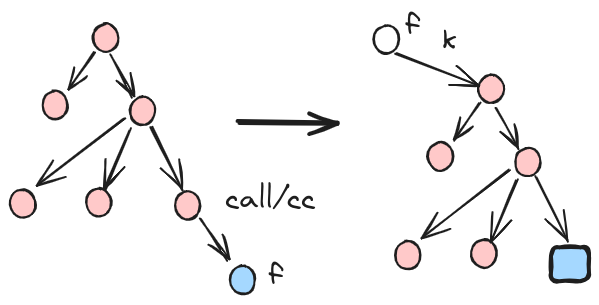
\includegraphics[width=0.6\linewidth]{/home/yukio/Diary/projs/fpcourse/fp-2024/docs/figs/call-cc}
    \caption{\texttt{call/cc} вызывает функцию \texttt{f} с продолжением \texttt{k}.
    Аргумент \texttt{k} подставляется вместо вхождения \texttt{call/cc}.}
    \label{fig:call-cc}
\end{figure}

\subsubsection{Continuation semantics}

Существует стиль формальных семантики, называемый \vocab{continuation semantics}.
Фактически он соответствует написанию определяющих интерпретаторов в CPS стиле.

% todo

\subsubsection{Эффективный CPS}

% todo kotlin

% todo rust

% todo C# generators

\subsection{Дефункционализация продолжений}

\cite{reynolds1972definitional}

% todo zipper

% todo abstract machines

% todo

\subsection{Delimited continuations}

\footnote{\url{https://www.cl.cam.ac.uk/teaching/2324/R277/handout-delimited-continuations.pdf}}

\cite{dyvbig2007monadic}

% todo in haskell

% todo via mutable cell (Representing Monads)

% todo Kotlin stack Jumps

% todo

\subsection{Нативная реализация продолжений}

\subsubsection{State machine}

% todo циклы и спиллинг

% todo

\subsubsection{Continuios stack}

% todo

\subsubsection{Segmented stack}

% todo

\subsection{Использование продолжений}

% todo difference lists

% todo lens

% todo CPS интерпретаторы, переходы

% todo корутины

% todo генераторы

% todo эффекты

% todo transducers, pipelines and internal iteration

% todo CEKT

% todo continuation semantics


% todo citations on operators

% todo continuations and operating systems

% todo origins: yoneda (reason isomorphically), logic

% todo continuations and imperative programming

% todo single-shot/multi-shot

% todo codensity

% todo problems with continuations: typing and resources

% todo implementing while & break

% todo

% todo control operator, runtime наизнанку


% todo coroutines example https://en.wikibooks.org/wiki/Haskell/Continuation_passing_style

% todo пример на хаскеле с примитивом


% todo goto не нужен?  


% todo Foundations for Programming and Implementing Effect Handlers

% todo sicp

% todo CPS трансформация интерпретаторов

% todo CPS correspond to double negation in logic reynolds1998definitional

% todo defuctionalized continuations, pepers from gibbons talk

% todo SPJ compiling without continuations

% todo difference lists

% todo The Essence of Cornpiling with Continuations

% todo calculating correct compilers

% todo reference to best refactoring
% todo refrence co calculate correct compilers and stuff

\cite{reynolds1972definitional, reynolds1998definitional, defunctionalization-slides}

% todo Oleg's web cite

% todo tags and prompts
